\documentclass[a4paper,12pt]{report}

\usepackage[french]{babel}

\usepackage[a4paper,top=2cm,bottom=2cm,left=3cm,right=3cm,marginparwidth=1.75cm]{geometry}

% Useful packages
\usepackage{amsmath, amsfonts, amssymb}
\usepackage{graphicx}
\usepackage{color}
\usepackage[colorlinks=true, allcolors=blue]{hyperref}
\usepackage{tikz}
\usepackage{pgfplots}
\pgfplotsset{compat=1.18}

\title{Rapport d'activités}
\author{Viet Anh QUACH}

\begin{document}
\maketitle
\tableofcontents

\setcounter{secnumdepth}{4}

\chapter{Introduction de la thèse}


\chapter{Bibliographie}
\section{MPM}
\begin{itemize}
\item Thèse: Application de la Méthode des Points Matériels aux phénomènes gravitaires - Fabio GRACIA DANIES
\item A multi-scale, MPMxDEM, numerical modelling approach for geotechnical structures under severe loading - Sacha Duverger
\item Material Point Method -- Vinh Phu NGUYEN, Alban de Vaucorbeil, Stephane Bordas
\end{itemize}
\section{DEM}
\begin{itemize}
      \item \cite{combe2023demlecture}
      \item Thèse: Modélisation multi-échelle des matériaux granulaires frottant-cohésifs: Trung Kien NGUYEN
\end{itemize}

\section{Couplage MPMxDEM}
\begin{itemize}
      \item Thèse: Application de la Méthode des Points Matériels aux phénomènes gravitaires - Fabio GRACIA DANIES
      \item \cite{richefeu2025mpmxdem}
\end{itemize}
\section{Corrélation}

\section{Compétences soutenues}
\begin{itemize}
      \item C++
      \item Gnuplot
      \item LaTeX
\end{itemize}

% Inkscape
% Writing thesis
% 120 formations sur ADUM
% Linux
% Clavier français :D

\chapter{L'étude pratique}
\section{Simulation MPM}
\subsection{Étude sur le cas statique - Déformation d'une poutre console}
\subsubsection{PIC}
\subsubsection{coefficient Poisson}
\subsubsection{Longueur encastrée}
\subsubsection{Discrétisation du maillage}
\subsubsection{Comparaison entre calcul théorique et numérique}
                                \begin{figure}
                                   \small % GNUPLOT: LaTeX picture with Postscript
\begingroup
  \makeatletter
  \providecommand\color[2][]{%
    \GenericError{(gnuplot) \space\space\space\@spaces}{%
      Package color not loaded in conjunction with
      terminal option `colourtext'%
    }{See the gnuplot documentation for explanation.%
    }{Either use 'blacktext' in gnuplot or load the package
      color.sty in LaTeX.}%
    \renewcommand\color[2][]{}%
  }%
  \providecommand\includegraphics[2][]{%
    \GenericError{(gnuplot) \space\space\space\@spaces}{%
      Package graphicx or graphics not loaded%
    }{See the gnuplot documentation for explanation.%
    }{The gnuplot epslatex terminal needs graphicx.sty or graphics.sty.}%
    \renewcommand\includegraphics[2][]{}%
  }%
  \providecommand\rotatebox[2]{#2}%
  \@ifundefined{ifGPcolor}{%
    \newif\ifGPcolor
    \GPcolortrue
  }{}%
  \@ifundefined{ifGPblacktext}{%
    \newif\ifGPblacktext
    \GPblacktextfalse
  }{}%
  % define a \g@addto@macro without @ in the name:
  \let\gplgaddtomacro\g@addto@macro
  % define empty templates for all commands taking text:
  \gdef\gplbacktext{}%
  \gdef\gplfronttext{}%
  \makeatother
  \ifGPblacktext
    % no textcolor at all
    \def\colorrgb#1{}%
    \def\colorgray#1{}%
  \else
    % gray or color?
    \ifGPcolor
      \def\colorrgb#1{\color[rgb]{#1}}%
      \def\colorgray#1{\color[gray]{#1}}%
      \expandafter\def\csname LTw\endcsname{\color{white}}%
      \expandafter\def\csname LTb\endcsname{\color{black}}%
      \expandafter\def\csname LTa\endcsname{\color{black}}%
      \expandafter\def\csname LT0\endcsname{\color[rgb]{1,0,0}}%
      \expandafter\def\csname LT1\endcsname{\color[rgb]{0,1,0}}%
      \expandafter\def\csname LT2\endcsname{\color[rgb]{0,0,1}}%
      \expandafter\def\csname LT3\endcsname{\color[rgb]{1,0,1}}%
      \expandafter\def\csname LT4\endcsname{\color[rgb]{0,1,1}}%
      \expandafter\def\csname LT5\endcsname{\color[rgb]{1,1,0}}%
      \expandafter\def\csname LT6\endcsname{\color[rgb]{0,0,0}}%
      \expandafter\def\csname LT7\endcsname{\color[rgb]{1,0.3,0}}%
      \expandafter\def\csname LT8\endcsname{\color[rgb]{0.5,0.5,0.5}}%
    \else
      % gray
      \def\colorrgb#1{\color{black}}%
      \def\colorgray#1{\color[gray]{#1}}%
      \expandafter\def\csname LTw\endcsname{\color{white}}%
      \expandafter\def\csname LTb\endcsname{\color{black}}%
      \expandafter\def\csname LTa\endcsname{\color{black}}%
      \expandafter\def\csname LT0\endcsname{\color{black}}%
      \expandafter\def\csname LT1\endcsname{\color{black}}%
      \expandafter\def\csname LT2\endcsname{\color{black}}%
      \expandafter\def\csname LT3\endcsname{\color{black}}%
      \expandafter\def\csname LT4\endcsname{\color{black}}%
      \expandafter\def\csname LT5\endcsname{\color{black}}%
      \expandafter\def\csname LT6\endcsname{\color{black}}%
      \expandafter\def\csname LT7\endcsname{\color{black}}%
      \expandafter\def\csname LT8\endcsname{\color{black}}%
    \fi
  \fi
    \setlength{\unitlength}{0.0500bp}%
    \ifx\gptboxheight\undefined%
      \newlength{\gptboxheight}%
      \newlength{\gptboxwidth}%
      \newsavebox{\gptboxtext}%
    \fi%
    \setlength{\fboxrule}{0.5pt}%
    \setlength{\fboxsep}{1pt}%
    \definecolor{tbcol}{rgb}{1,1,1}%
\begin{picture}(7200.00,5040.00)%
    \gplgaddtomacro\gplbacktext{%
      \csname LTb\endcsname%%
      \put(682,704){\makebox(0,0)[r]{\strut{}$-5$}}%
      \csname LTb\endcsname%%
      \put(682,1390){\makebox(0,0)[r]{\strut{}$-4$}}%
      \csname LTb\endcsname%%
      \put(682,2076){\makebox(0,0)[r]{\strut{}$-3$}}%
      \csname LTb\endcsname%%
      \put(682,2762){\makebox(0,0)[r]{\strut{}$-2$}}%
      \csname LTb\endcsname%%
      \put(682,3447){\makebox(0,0)[r]{\strut{}$-1$}}%
      \csname LTb\endcsname%%
      \put(682,4133){\makebox(0,0)[r]{\strut{}$0$}}%
      \csname LTb\endcsname%%
      \put(682,4819){\makebox(0,0)[r]{\strut{}$1$}}%
      \csname LTb\endcsname%%
      \put(814,484){\makebox(0,0){\strut{}$0$}}%
      \csname LTb\endcsname%%
      \put(2012,484){\makebox(0,0){\strut{}$0.2$}}%
      \csname LTb\endcsname%%
      \put(3210,484){\makebox(0,0){\strut{}$0.4$}}%
      \csname LTb\endcsname%%
      \put(4407,484){\makebox(0,0){\strut{}$0.6$}}%
      \csname LTb\endcsname%%
      \put(5605,484){\makebox(0,0){\strut{}$0.8$}}%
      \csname LTb\endcsname%%
      \put(6803,484){\makebox(0,0){\strut{}$1$}}%
    }%
    \gplgaddtomacro\gplfronttext{%
      \csname LTb\endcsname%%
      \put(209,2761){\rotatebox{-270}{\makebox(0,0){\strut{}$f_y$ (mm)}}}%
      \put(3808,154){\makebox(0,0){\strut{}$x$ (m)}}%
      \csname LTb\endcsname%%
      \put(6009,4493){\makebox(0,0)[r]{\strut{}$\text{f}_{\text{calcul}}$}}%
      \csname LTb\endcsname%%
      \put(6009,4373){\makebox(0,0)[r]{\strut{}$\text{f}_{\text{théorique}}$}}%
      \csname LTb\endcsname%%
      \put(3808,33733){\makebox(0,0){\strut{}}}%
    }%
    \gplbacktext
    \put(0,0){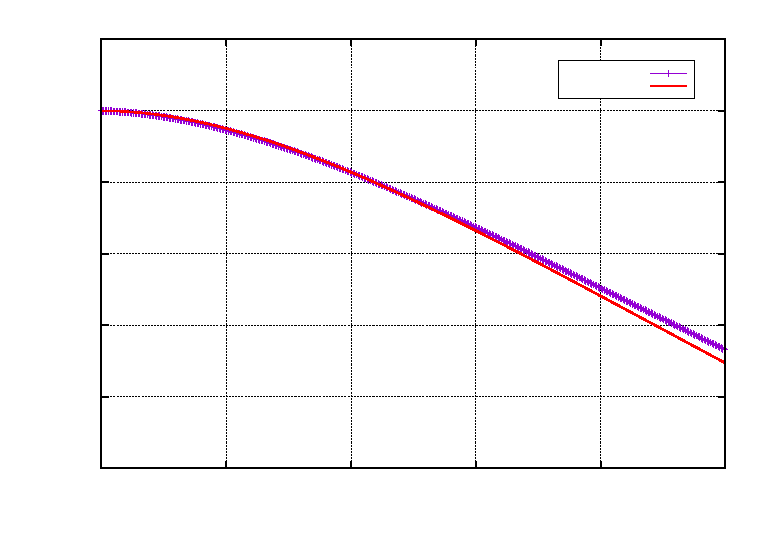
\includegraphics[width={360.00bp},height={252.00bp}]{./Deplacement_Poutre}}%
    \gplfronttext
  \end{picture}%
\endgroup

                                    \caption{Déplacement du poutre en Y-axis}
                                \end{figure}
\subsection{Étude sur le cas dynamique}


\section{Simulation DEM: Compression triaxiale}
\subsection{Le processus et les paramètres}
\subsection{Les caractéristiques mécaniques générales du sol}
\subsubsection{La granulométrie et la fraction solide}
\subsubsection{La granulométrie et la fraction solide}
\subsubsection{Les caractéristiques des échantillons denses}
\subsubsection{Les caractéristiques des échantillons lâches}
\subsubsection{L'état critique}
\paragraph{La force entre les grains}
\paragraph{L'indice de vide}
\paragraph{Le nombre de coordination}
\subsubsection{Cercle de Mohr}
\subsubsection{Histoire du chargement}

\subsection{Recherche sur l'impact dynamique}

\subsubsection{Augmentation du nombre d'inertie (Montée la vitesse imposée)}
\begin{figure}
\centering
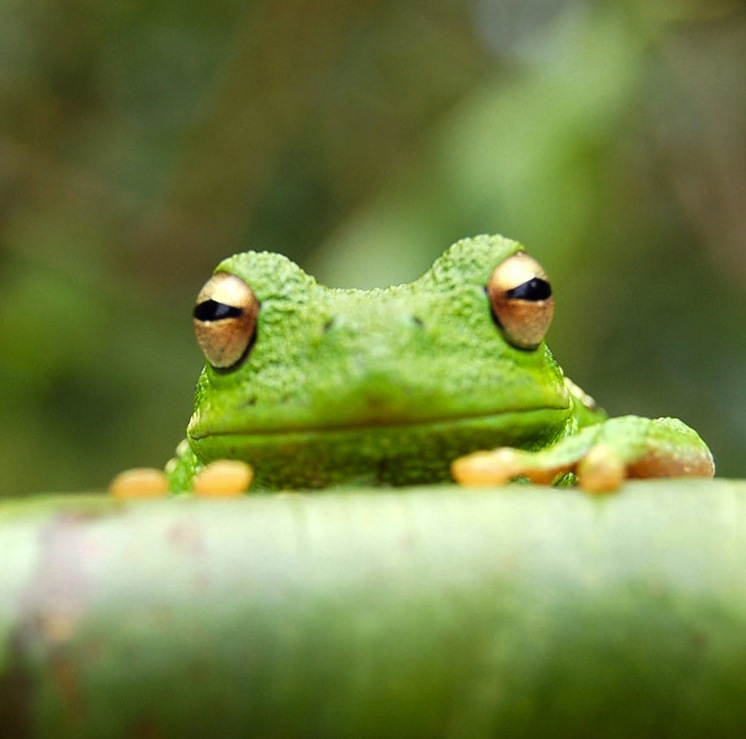
\includegraphics[width=0.3\textwidth]{frog.jpg}
\caption{\label{fig:frog}This frog was uploaded via the file-tree menu.}
\end{figure}

\section{Couplage\ldots}
\subsection{How to add Tables}

Use the table and tabular environments for basic tables --- see Table~\ref{tab:widgets}, for example. For more information, please see this help article on \href{https://www.overleaf.com/learn/latex/tables}{tables}. 

\begin{table}
\centering
\begin{tabular}{l|r}
Item & Quantity \\\hline
Widgets & 42 \\
Gadgets & 13
\end{tabular}
\caption{\label{tab:widgets}An example table.}
\end{table}

\subsection{How to add Lists}

You can make lists with automatic numbering \dots

\begin{enumerate}
\item Like this,
\item and like this.
\end{enumerate}
\dots or bullet points \dots
\begin{itemize}
\item Like this,
\item and like this.
\end{itemize}
\chapter{Conclusion}

                                \begin{figure}
                                  \small
                                  % GNUPLOT: LaTeX picture with Postscript
\begingroup
  \makeatletter
  \providecommand\color[2][]{%
    \GenericError{(gnuplot) \space\space\space\@spaces}{%
      Package color not loaded in conjunction with
      terminal option `colourtext'%
    }{See the gnuplot documentation for explanation.%
    }{Either use 'blacktext' in gnuplot or load the package
      color.sty in LaTeX.}%
    \renewcommand\color[2][]{}%
  }%
  \providecommand\includegraphics[2][]{%
    \GenericError{(gnuplot) \space\space\space\@spaces}{%
      Package graphicx or graphics not loaded%
    }{See the gnuplot documentation for explanation.%
    }{The gnuplot epslatex terminal needs graphicx.sty or graphics.sty.}%
    \renewcommand\includegraphics[2][]{}%
  }%
  \providecommand\rotatebox[2]{#2}%
  \@ifundefined{ifGPcolor}{%
    \newif\ifGPcolor
    \GPcolortrue
  }{}%
  \@ifundefined{ifGPblacktext}{%
    \newif\ifGPblacktext
    \GPblacktextfalse
  }{}%
  % define a \g@addto@macro without @ in the name:
  \let\gplgaddtomacro\g@addto@macro
  % define empty templates for all commands taking text:
  \gdef\gplbacktext{}%
  \gdef\gplfronttext{}%
  \makeatother
  \ifGPblacktext
    % no textcolor at all
    \def\colorrgb#1{}%
    \def\colorgray#1{}%
  \else
    % gray or color?
    \ifGPcolor
      \def\colorrgb#1{\color[rgb]{#1}}%
      \def\colorgray#1{\color[gray]{#1}}%
      \expandafter\def\csname LTw\endcsname{\color{white}}%
      \expandafter\def\csname LTb\endcsname{\color{black}}%
      \expandafter\def\csname LTa\endcsname{\color{black}}%
      \expandafter\def\csname LT0\endcsname{\color[rgb]{1,0,0}}%
      \expandafter\def\csname LT1\endcsname{\color[rgb]{0,1,0}}%
      \expandafter\def\csname LT2\endcsname{\color[rgb]{0,0,1}}%
      \expandafter\def\csname LT3\endcsname{\color[rgb]{1,0,1}}%
      \expandafter\def\csname LT4\endcsname{\color[rgb]{0,1,1}}%
      \expandafter\def\csname LT5\endcsname{\color[rgb]{1,1,0}}%
      \expandafter\def\csname LT6\endcsname{\color[rgb]{0,0,0}}%
      \expandafter\def\csname LT7\endcsname{\color[rgb]{1,0.3,0}}%
      \expandafter\def\csname LT8\endcsname{\color[rgb]{0.5,0.5,0.5}}%
    \else
      % gray
      \def\colorrgb#1{\color{black}}%
      \def\colorgray#1{\color[gray]{#1}}%
      \expandafter\def\csname LTw\endcsname{\color{white}}%
      \expandafter\def\csname LTb\endcsname{\color{black}}%
      \expandafter\def\csname LTa\endcsname{\color{black}}%
      \expandafter\def\csname LT0\endcsname{\color{black}}%
      \expandafter\def\csname LT1\endcsname{\color{black}}%
      \expandafter\def\csname LT2\endcsname{\color{black}}%
      \expandafter\def\csname LT3\endcsname{\color{black}}%
      \expandafter\def\csname LT4\endcsname{\color{black}}%
      \expandafter\def\csname LT5\endcsname{\color{black}}%
      \expandafter\def\csname LT6\endcsname{\color{black}}%
      \expandafter\def\csname LT7\endcsname{\color{black}}%
      \expandafter\def\csname LT8\endcsname{\color{black}}%
    \fi
  \fi
    \setlength{\unitlength}{0.0500bp}%
    \ifx\gptboxheight\undefined%
      \newlength{\gptboxheight}%
      \newlength{\gptboxwidth}%
      \newsavebox{\gptboxtext}%
    \fi%
    \setlength{\fboxrule}{0.5pt}%
    \setlength{\fboxsep}{1pt}%
    \definecolor{tbcol}{rgb}{1,1,1}%
\begin{picture}(7200.00,5040.00)%
    \gplgaddtomacro\gplbacktext{%
      \csname LTb\endcsname%%
      \put(946,1834){\makebox(0,0)[r]{\strut{}$0.62$}}%
      \csname LTb\endcsname%%
      \put(946,2293){\makebox(0,0)[r]{\strut{}$0.64$}}%
      \csname LTb\endcsname%%
      \put(946,2752){\makebox(0,0)[r]{\strut{}$0.66$}}%
      \csname LTb\endcsname%%
      \put(946,3212){\makebox(0,0)[r]{\strut{}$0.68$}}%
      \csname LTb\endcsname%%
      \put(946,3671){\makebox(0,0)[r]{\strut{}$0.7$}}%
      \csname LTb\endcsname%%
      \put(946,4130){\makebox(0,0)[r]{\strut{}$0.72$}}%
      \csname LTb\endcsname%%
      \put(946,4589){\makebox(0,0)[r]{\strut{}$0.74$}}%
      \csname LTb\endcsname%%
      \put(1078,1384){\makebox(0,0){\strut{}$0$}}%
      \csname LTb\endcsname%%
      \put(2223,1384){\makebox(0,0){\strut{}$20$}}%
      \csname LTb\endcsname%%
      \put(3368,1384){\makebox(0,0){\strut{}$40$}}%
      \csname LTb\endcsname%%
      \put(4513,1384){\makebox(0,0){\strut{}$60$}}%
      \csname LTb\endcsname%%
      \put(5658,1384){\makebox(0,0){\strut{}$80$}}%
      \csname LTb\endcsname%%
      \put(6803,1384){\makebox(0,0){\strut{}$100$}}%
    }%
    \gplgaddtomacro\gplfronttext{%
      \csname LTb\endcsname%%
      \put(209,3211){\rotatebox{-270}{\makebox(0,0){\strut{}e}}}%
      \put(3940,1054){\makebox(0,0){\strut{}$\varepsilon_{yy}$ (\%)}}%
      \csname LTb\endcsname%%
      \put(2046,813){\makebox(0,0)[r]{\strut{}$I = 1 \times 10^{-4}$}}%
      \csname LTb\endcsname%%
      \put(2046,513){\makebox(0,0)[r]{\strut{}$I = 1 \times 10^{-3}$}}%
      \csname LTb\endcsname%%
      \put(2046,213){\makebox(0,0)[r]{\strut{}$I = 2 \times 10^{-3}$}}%
      \csname LTb\endcsname%%
      \put(4269,813){\makebox(0,0)[r]{\strut{}$I = 4 \times 10^{-3}$}}%
      \csname LTb\endcsname%%
      \put(4269,513){\makebox(0,0)[r]{\strut{}$I = 6 \times 10^{-3}$}}%
      \csname LTb\endcsname%%
      \put(4269,213){\makebox(0,0)[r]{\strut{}$I = 8 \times 10^{-3}$}}%
      \csname LTb\endcsname%%
      \put(6492,813){\makebox(0,0)[r]{\strut{}$I = 1 \times 10^{-2}$}}%
    }%
    \gplbacktext
    \put(0,0){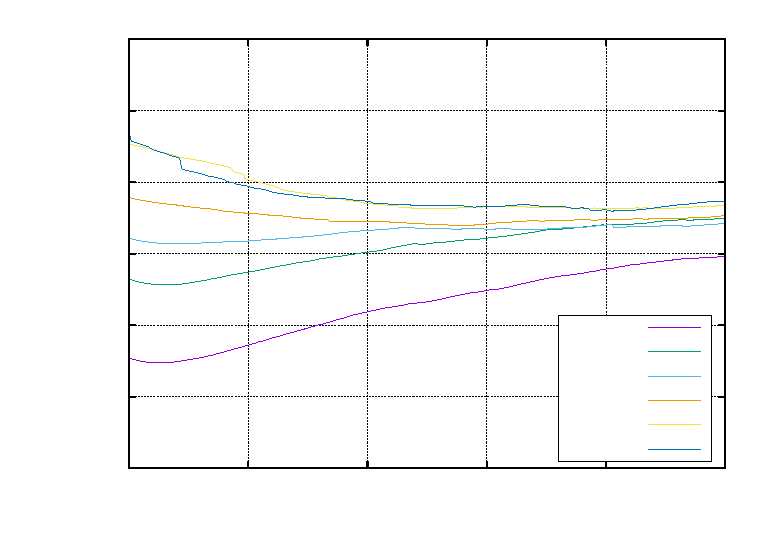
\includegraphics[width={360.00bp},height={252.00bp}]{./RapportVides}}%
    \gplfronttext
  \end{picture}%
\endgroup

                                    \caption{L'indice de vide}
                                \end{figure}
                                    
                                \begin{figure}
                                   % GNUPLOT: LaTeX picture with Postscript
\begingroup
  \makeatletter
  \providecommand\color[2][]{%
    \GenericError{(gnuplot) \space\space\space\@spaces}{%
      Package color not loaded in conjunction with
      terminal option `colourtext'%
    }{See the gnuplot documentation for explanation.%
    }{Either use 'blacktext' in gnuplot or load the package
      color.sty in LaTeX.}%
    \renewcommand\color[2][]{}%
  }%
  \providecommand\includegraphics[2][]{%
    \GenericError{(gnuplot) \space\space\space\@spaces}{%
      Package graphicx or graphics not loaded%
    }{See the gnuplot documentation for explanation.%
    }{The gnuplot epslatex terminal needs graphicx.sty or graphics.sty.}%
    \renewcommand\includegraphics[2][]{}%
  }%
  \providecommand\rotatebox[2]{#2}%
  \@ifundefined{ifGPcolor}{%
    \newif\ifGPcolor
    \GPcolortrue
  }{}%
  \@ifundefined{ifGPblacktext}{%
    \newif\ifGPblacktext
    \GPblacktextfalse
  }{}%
  % define a \g@addto@macro without @ in the name:
  \let\gplgaddtomacro\g@addto@macro
  % define empty templates for all commands taking text:
  \gdef\gplbacktext{}%
  \gdef\gplfronttext{}%
  \makeatother
  \ifGPblacktext
    % no textcolor at all
    \def\colorrgb#1{}%
    \def\colorgray#1{}%
  \else
    % gray or color?
    \ifGPcolor
      \def\colorrgb#1{\color[rgb]{#1}}%
      \def\colorgray#1{\color[gray]{#1}}%
      \expandafter\def\csname LTw\endcsname{\color{white}}%
      \expandafter\def\csname LTb\endcsname{\color{black}}%
      \expandafter\def\csname LTa\endcsname{\color{black}}%
      \expandafter\def\csname LT0\endcsname{\color[rgb]{1,0,0}}%
      \expandafter\def\csname LT1\endcsname{\color[rgb]{0,1,0}}%
      \expandafter\def\csname LT2\endcsname{\color[rgb]{0,0,1}}%
      \expandafter\def\csname LT3\endcsname{\color[rgb]{1,0,1}}%
      \expandafter\def\csname LT4\endcsname{\color[rgb]{0,1,1}}%
      \expandafter\def\csname LT5\endcsname{\color[rgb]{1,1,0}}%
      \expandafter\def\csname LT6\endcsname{\color[rgb]{0,0,0}}%
      \expandafter\def\csname LT7\endcsname{\color[rgb]{1,0.3,0}}%
      \expandafter\def\csname LT8\endcsname{\color[rgb]{0.5,0.5,0.5}}%
    \else
      % gray
      \def\colorrgb#1{\color{black}}%
      \def\colorgray#1{\color[gray]{#1}}%
      \expandafter\def\csname LTw\endcsname{\color{white}}%
      \expandafter\def\csname LTb\endcsname{\color{black}}%
      \expandafter\def\csname LTa\endcsname{\color{black}}%
      \expandafter\def\csname LT0\endcsname{\color{black}}%
      \expandafter\def\csname LT1\endcsname{\color{black}}%
      \expandafter\def\csname LT2\endcsname{\color{black}}%
      \expandafter\def\csname LT3\endcsname{\color{black}}%
      \expandafter\def\csname LT4\endcsname{\color{black}}%
      \expandafter\def\csname LT5\endcsname{\color{black}}%
      \expandafter\def\csname LT6\endcsname{\color{black}}%
      \expandafter\def\csname LT7\endcsname{\color{black}}%
      \expandafter\def\csname LT8\endcsname{\color{black}}%
    \fi
  \fi
    \setlength{\unitlength}{0.0500bp}%
    \ifx\gptboxheight\undefined%
      \newlength{\gptboxheight}%
      \newlength{\gptboxwidth}%
      \newsavebox{\gptboxtext}%
    \fi%
    \setlength{\fboxrule}{0.5pt}%
    \setlength{\fboxsep}{1pt}%
    \definecolor{tbcol}{rgb}{1,1,1}%
\begin{picture}(7200.00,5040.00)%
    \gplgaddtomacro\gplbacktext{%
      \csname LTb\endcsname%%
      \put(814,1604){\makebox(0,0)[r]{\strut{}$1$}}%
      \csname LTb\endcsname%%
      \put(814,1961){\makebox(0,0)[r]{\strut{}$1.5$}}%
      \csname LTb\endcsname%%
      \put(814,2318){\makebox(0,0)[r]{\strut{}$2$}}%
      \csname LTb\endcsname%%
      \put(814,2676){\makebox(0,0)[r]{\strut{}$2.5$}}%
      \csname LTb\endcsname%%
      \put(814,3033){\makebox(0,0)[r]{\strut{}$3$}}%
      \csname LTb\endcsname%%
      \put(814,3390){\makebox(0,0)[r]{\strut{}$3.5$}}%
      \csname LTb\endcsname%%
      \put(814,3747){\makebox(0,0)[r]{\strut{}$4$}}%
      \csname LTb\endcsname%%
      \put(814,4105){\makebox(0,0)[r]{\strut{}$4.5$}}%
      \csname LTb\endcsname%%
      \put(814,4462){\makebox(0,0)[r]{\strut{}$5$}}%
      \csname LTb\endcsname%%
      \put(814,4819){\makebox(0,0)[r]{\strut{}$5.5$}}%
      \csname LTb\endcsname%%
      \put(946,1384){\makebox(0,0){\strut{}$0$}}%
      \csname LTb\endcsname%%
      \put(2117,1384){\makebox(0,0){\strut{}$20$}}%
      \csname LTb\endcsname%%
      \put(3289,1384){\makebox(0,0){\strut{}$40$}}%
      \csname LTb\endcsname%%
      \put(4460,1384){\makebox(0,0){\strut{}$60$}}%
      \csname LTb\endcsname%%
      \put(5632,1384){\makebox(0,0){\strut{}$80$}}%
      \csname LTb\endcsname%%
      \put(6803,1384){\makebox(0,0){\strut{}$100$}}%
    }%
    \gplgaddtomacro\gplfronttext{%
      \csname LTb\endcsname%%
      \put(209,3211){\rotatebox{-270}{\makebox(0,0){\strut{}Z}}}%
      \put(3874,1054){\makebox(0,0){\strut{}$\varepsilon_{yy}$ (\%)}}%
      \csname LTb\endcsname%%
      \put(1980,813){\makebox(0,0)[r]{\strut{}$I = 1 \times 10^{-4}$}}%
      \csname LTb\endcsname%%
      \put(1980,513){\makebox(0,0)[r]{\strut{}$I = 1 \times 10^{-3}$}}%
      \csname LTb\endcsname%%
      \put(1980,213){\makebox(0,0)[r]{\strut{}$I = 2 \times 10^{-3}$}}%
      \csname LTb\endcsname%%
      \put(4203,813){\makebox(0,0)[r]{\strut{}$I = 4 \times 10^{-3}$}}%
      \csname LTb\endcsname%%
      \put(4203,513){\makebox(0,0)[r]{\strut{}$I = 6 \times 10^{-3}$}}%
      \csname LTb\endcsname%%
      \put(4203,213){\makebox(0,0)[r]{\strut{}$I = 8 \times 10^{-3}$}}%
      \csname LTb\endcsname%%
      \put(6426,813){\makebox(0,0)[r]{\strut{}$I = 1 \times 10^{-2}$}}%
    }%
    \gplbacktext
    \put(0,0){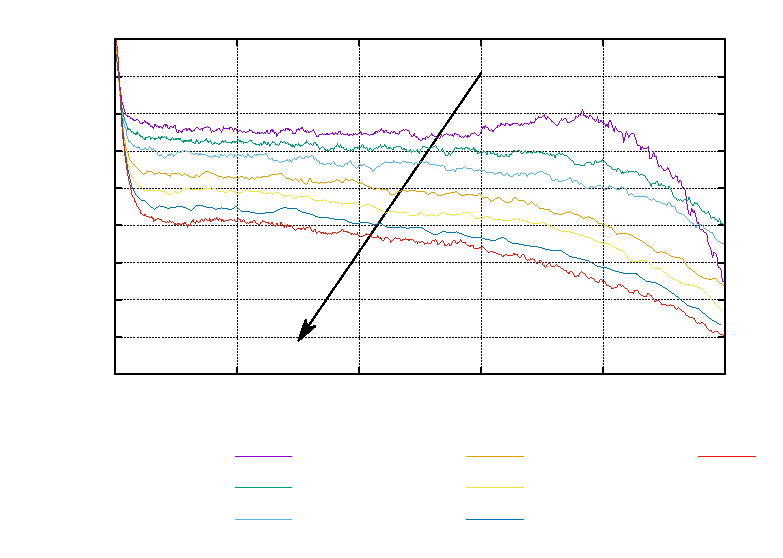
\includegraphics[width={360.00bp},height={252.00bp}]{./NombreCoordination}}%
    \gplfronttext
  \end{picture}%
\endgroup

                                    \caption{Nombre de coordination}
                                \end{figure}

                                Vitesse imposée est élevée $\rightarrow$ Contrainte de confinement et l'indice de vide sont instables

     
                                \begin{figure}
                                    % GNUPLOT: LaTeX picture with Postscript
\begingroup
  \makeatletter
  \providecommand\color[2][]{%
    \GenericError{(gnuplot) \space\space\space\@spaces}{%
      Package color not loaded in conjunction with
      terminal option `colourtext'%
    }{See the gnuplot documentation for explanation.%
    }{Either use 'blacktext' in gnuplot or load the package
      color.sty in LaTeX.}%
    \renewcommand\color[2][]{}%
  }%
  \providecommand\includegraphics[2][]{%
    \GenericError{(gnuplot) \space\space\space\@spaces}{%
      Package graphicx or graphics not loaded%
    }{See the gnuplot documentation for explanation.%
    }{The gnuplot epslatex terminal needs graphicx.sty or graphics.sty.}%
    \renewcommand\includegraphics[2][]{}%
  }%
  \providecommand\rotatebox[2]{#2}%
  \@ifundefined{ifGPcolor}{%
    \newif\ifGPcolor
    \GPcolortrue
  }{}%
  \@ifundefined{ifGPblacktext}{%
    \newif\ifGPblacktext
    \GPblacktextfalse
  }{}%
  % define a \g@addto@macro without @ in the name:
  \let\gplgaddtomacro\g@addto@macro
  % define empty templates for all commands taking text:
  \gdef\gplbacktext{}%
  \gdef\gplfronttext{}%
  \makeatother
  \ifGPblacktext
    % no textcolor at all
    \def\colorrgb#1{}%
    \def\colorgray#1{}%
  \else
    % gray or color?
    \ifGPcolor
      \def\colorrgb#1{\color[rgb]{#1}}%
      \def\colorgray#1{\color[gray]{#1}}%
      \expandafter\def\csname LTw\endcsname{\color{white}}%
      \expandafter\def\csname LTb\endcsname{\color{black}}%
      \expandafter\def\csname LTa\endcsname{\color{black}}%
      \expandafter\def\csname LT0\endcsname{\color[rgb]{1,0,0}}%
      \expandafter\def\csname LT1\endcsname{\color[rgb]{0,1,0}}%
      \expandafter\def\csname LT2\endcsname{\color[rgb]{0,0,1}}%
      \expandafter\def\csname LT3\endcsname{\color[rgb]{1,0,1}}%
      \expandafter\def\csname LT4\endcsname{\color[rgb]{0,1,1}}%
      \expandafter\def\csname LT5\endcsname{\color[rgb]{1,1,0}}%
      \expandafter\def\csname LT6\endcsname{\color[rgb]{0,0,0}}%
      \expandafter\def\csname LT7\endcsname{\color[rgb]{1,0.3,0}}%
      \expandafter\def\csname LT8\endcsname{\color[rgb]{0.5,0.5,0.5}}%
    \else
      % gray
      \def\colorrgb#1{\color{black}}%
      \def\colorgray#1{\color[gray]{#1}}%
      \expandafter\def\csname LTw\endcsname{\color{white}}%
      \expandafter\def\csname LTb\endcsname{\color{black}}%
      \expandafter\def\csname LTa\endcsname{\color{black}}%
      \expandafter\def\csname LT0\endcsname{\color{black}}%
      \expandafter\def\csname LT1\endcsname{\color{black}}%
      \expandafter\def\csname LT2\endcsname{\color{black}}%
      \expandafter\def\csname LT3\endcsname{\color{black}}%
      \expandafter\def\csname LT4\endcsname{\color{black}}%
      \expandafter\def\csname LT5\endcsname{\color{black}}%
      \expandafter\def\csname LT6\endcsname{\color{black}}%
      \expandafter\def\csname LT7\endcsname{\color{black}}%
      \expandafter\def\csname LT8\endcsname{\color{black}}%
    \fi
  \fi
    \setlength{\unitlength}{0.0500bp}%
    \ifx\gptboxheight\undefined%
      \newlength{\gptboxheight}%
      \newlength{\gptboxwidth}%
      \newsavebox{\gptboxtext}%
    \fi%
    \setlength{\fboxrule}{0.5pt}%
    \setlength{\fboxsep}{1pt}%
    \definecolor{tbcol}{rgb}{1,1,1}%
\begin{picture}(7200.00,5040.00)%
    \gplgaddtomacro\gplbacktext{%
      \csname LTb\endcsname%%
      \put(946,1584){\makebox(0,0)[r]{\strut{}$0$}}%
      \csname LTb\endcsname%%
      \put(946,2123){\makebox(0,0)[r]{\strut{}$200$}}%
      \csname LTb\endcsname%%
      \put(946,2662){\makebox(0,0)[r]{\strut{}$400$}}%
      \csname LTb\endcsname%%
      \put(946,3202){\makebox(0,0)[r]{\strut{}$600$}}%
      \csname LTb\endcsname%%
      \put(946,3741){\makebox(0,0)[r]{\strut{}$800$}}%
      \csname LTb\endcsname%%
      \put(946,4280){\makebox(0,0)[r]{\strut{}$1000$}}%
      \csname LTb\endcsname%%
      \put(946,4819){\makebox(0,0)[r]{\strut{}$1200$}}%
      \csname LTb\endcsname%%
      \put(1078,1364){\makebox(0,0){\strut{}$0$}}%
      \csname LTb\endcsname%%
      \put(1700,1364){\makebox(0,0){\strut{}$10$}}%
      \csname LTb\endcsname%%
      \put(2322,1364){\makebox(0,0){\strut{}$20$}}%
      \csname LTb\endcsname%%
      \put(2944,1364){\makebox(0,0){\strut{}$30$}}%
      \csname LTb\endcsname%%
      \put(3567,1364){\makebox(0,0){\strut{}$40$}}%
      \csname LTb\endcsname%%
      \put(4189,1364){\makebox(0,0){\strut{}$50$}}%
      \csname LTb\endcsname%%
      \put(4811,1364){\makebox(0,0){\strut{}$60$}}%
      \csname LTb\endcsname%%
      \put(5433,1364){\makebox(0,0){\strut{}$70$}}%
      \csname LTb\endcsname%%
      \put(6055,1364){\makebox(0,0){\strut{}$80$}}%
      \put(6187,1584){\makebox(0,0)[l]{\strut{}$-2$}}%
      \put(6187,1908){\makebox(0,0)[l]{\strut{}$-1$}}%
      \put(6187,2231){\makebox(0,0)[l]{\strut{}$0$}}%
      \put(6187,2555){\makebox(0,0)[l]{\strut{}$1$}}%
      \put(6187,2878){\makebox(0,0)[l]{\strut{}$2$}}%
      \put(6187,3202){\makebox(0,0)[l]{\strut{}$3$}}%
      \put(6187,3525){\makebox(0,0)[l]{\strut{}$4$}}%
      \put(6187,3849){\makebox(0,0)[l]{\strut{}$5$}}%
      \put(6187,4172){\makebox(0,0)[l]{\strut{}$6$}}%
      \put(6187,4496){\makebox(0,0)[l]{\strut{}$7$}}%
      \put(6187,4819){\makebox(0,0)[l]{\strut{}$8$}}%
    }%
    \gplgaddtomacro\gplfronttext{%
      \csname LTb\endcsname%%
      \put(341,3201){\rotatebox{-270}{\makebox(0,0){\strut{}q (kPa)}}}%
      \put(6693,3201){\rotatebox{-270}{\makebox(0,0){\strut{}$\varepsilon_v$ (\%)}}}%
      \put(3566,1034){\makebox(0,0){\strut{}$\varepsilon_{yy}$ (\%)}}%
      \csname LTb\endcsname%%
      \put(2711,833){\makebox(0,0)[r]{\strut{}$I = 1 \times 10^{-4}$}}%
      \csname LTb\endcsname%%
      \put(2711,613){\makebox(0,0)[r]{\strut{}$I = 1 \times 10^{-3}$}}%
      \csname LTb\endcsname%%
      \put(2711,393){\makebox(0,0)[r]{\strut{}$I = 2 \times 10^{-3}$}}%
      \csname LTb\endcsname%%
      \put(2711,173){\makebox(0,0)[r]{\strut{}$I = 4 \times 10^{-3}$}}%
      \csname LTb\endcsname%%
      \put(5150,833){\makebox(0,0)[r]{\strut{}$I = 6 \times 10^{-3}$}}%
      \csname LTb\endcsname%%
      \put(5150,613){\makebox(0,0)[r]{\strut{}$I = 8 \times 10^{-3}$}}%
      \csname LTb\endcsname%%
      \put(5150,393){\makebox(0,0)[r]{\strut{}$I = 1 \times 10^{-2}$}}%
    }%
    \gplbacktext
    \put(0,0){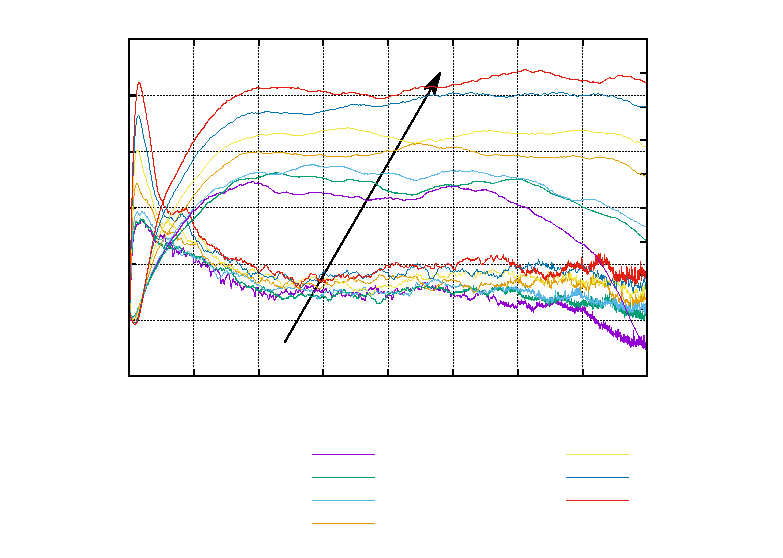
\includegraphics[width={360.00bp},height={252.00bp}]{./Test}}%
    \gplfronttext
  \end{picture}%
\endgroup

                                    \caption{Contrainte-Déformation}
                                \end{figure}
                                J'ai choisi $\varepsilon_{yy} = 70\%$ pour réaliser des pré-études sur la rhéologie $\mu(I)$ (considéré comme l'état critique). 


                                \begin{figure}
                                  % GNUPLOT: LaTeX picture with Postscript
\begingroup
  \makeatletter
  \providecommand\color[2][]{%
    \GenericError{(gnuplot) \space\space\space\@spaces}{%
      Package color not loaded in conjunction with
      terminal option `colourtext'%
    }{See the gnuplot documentation for explanation.%
    }{Either use 'blacktext' in gnuplot or load the package
      color.sty in LaTeX.}%
    \renewcommand\color[2][]{}%
  }%
  \providecommand\includegraphics[2][]{%
    \GenericError{(gnuplot) \space\space\space\@spaces}{%
      Package graphicx or graphics not loaded%
    }{See the gnuplot documentation for explanation.%
    }{The gnuplot epslatex terminal needs graphicx.sty or graphics.sty.}%
    \renewcommand\includegraphics[2][]{}%
  }%
  \providecommand\rotatebox[2]{#2}%
  \@ifundefined{ifGPcolor}{%
    \newif\ifGPcolor
    \GPcolortrue
  }{}%
  \@ifundefined{ifGPblacktext}{%
    \newif\ifGPblacktext
    \GPblacktextfalse
  }{}%
  % define a \g@addto@macro without @ in the name:
  \let\gplgaddtomacro\g@addto@macro
  % define empty templates for all commands taking text:
  \gdef\gplbacktext{}%
  \gdef\gplfronttext{}%
  \makeatother
  \ifGPblacktext
    % no textcolor at all
    \def\colorrgb#1{}%
    \def\colorgray#1{}%
  \else
    % gray or color?
    \ifGPcolor
      \def\colorrgb#1{\color[rgb]{#1}}%
      \def\colorgray#1{\color[gray]{#1}}%
      \expandafter\def\csname LTw\endcsname{\color{white}}%
      \expandafter\def\csname LTb\endcsname{\color{black}}%
      \expandafter\def\csname LTa\endcsname{\color{black}}%
      \expandafter\def\csname LT0\endcsname{\color[rgb]{1,0,0}}%
      \expandafter\def\csname LT1\endcsname{\color[rgb]{0,1,0}}%
      \expandafter\def\csname LT2\endcsname{\color[rgb]{0,0,1}}%
      \expandafter\def\csname LT3\endcsname{\color[rgb]{1,0,1}}%
      \expandafter\def\csname LT4\endcsname{\color[rgb]{0,1,1}}%
      \expandafter\def\csname LT5\endcsname{\color[rgb]{1,1,0}}%
      \expandafter\def\csname LT6\endcsname{\color[rgb]{0,0,0}}%
      \expandafter\def\csname LT7\endcsname{\color[rgb]{1,0.3,0}}%
      \expandafter\def\csname LT8\endcsname{\color[rgb]{0.5,0.5,0.5}}%
    \else
      % gray
      \def\colorrgb#1{\color{black}}%
      \def\colorgray#1{\color[gray]{#1}}%
      \expandafter\def\csname LTw\endcsname{\color{white}}%
      \expandafter\def\csname LTb\endcsname{\color{black}}%
      \expandafter\def\csname LTa\endcsname{\color{black}}%
      \expandafter\def\csname LT0\endcsname{\color{black}}%
      \expandafter\def\csname LT1\endcsname{\color{black}}%
      \expandafter\def\csname LT2\endcsname{\color{black}}%
      \expandafter\def\csname LT3\endcsname{\color{black}}%
      \expandafter\def\csname LT4\endcsname{\color{black}}%
      \expandafter\def\csname LT5\endcsname{\color{black}}%
      \expandafter\def\csname LT6\endcsname{\color{black}}%
      \expandafter\def\csname LT7\endcsname{\color{black}}%
      \expandafter\def\csname LT8\endcsname{\color{black}}%
    \fi
  \fi
    \setlength{\unitlength}{0.0500bp}%
    \ifx\gptboxheight\undefined%
      \newlength{\gptboxheight}%
      \newlength{\gptboxwidth}%
      \newsavebox{\gptboxtext}%
    \fi%
    \setlength{\fboxrule}{0.5pt}%
    \setlength{\fboxsep}{1pt}%
    \definecolor{tbcol}{rgb}{1,1,1}%
\begin{picture}(7200.00,5040.00)%
    \gplgaddtomacro\gplbacktext{%
      \csname LTb\endcsname%%
      \put(814,1881){\makebox(0,0)[r]{\strut{}$0$}}%
      \put(814,2299){\makebox(0,0)[r]{\strut{}$100$}}%
      \put(814,2718){\makebox(0,0)[r]{\strut{}$200$}}%
      \put(814,3136){\makebox(0,0)[r]{\strut{}$300$}}%
      \put(814,3554){\makebox(0,0)[r]{\strut{}$400$}}%
      \put(814,3973){\makebox(0,0)[r]{\strut{}$500$}}%
      \put(946,1661){\makebox(0,0){\strut{}$0$}}%
      \put(1783,1661){\makebox(0,0){\strut{}$200$}}%
      \put(2619,1661){\makebox(0,0){\strut{}$400$}}%
      \put(3456,1661){\makebox(0,0){\strut{}$600$}}%
      \put(4293,1661){\makebox(0,0){\strut{}$800$}}%
      \put(5130,1661){\makebox(0,0){\strut{}$1000$}}%
      \put(5966,1661){\makebox(0,0){\strut{}$1200$}}%
      \put(6803,1661){\makebox(0,0){\strut{}$1400$}}%
    }%
    \gplgaddtomacro\gplfronttext{%
      \csname LTb\endcsname%%
      \put(209,3031){\rotatebox{-270}{\makebox(0,0){\strut{}$\tau$ (kPa)}}}%
      \put(3874,1331){\makebox(0,0){\strut{}$\sigma_n$ (kPa)}}%
      \csname LTb\endcsname%%
      \put(2160,513){\makebox(0,0)[r]{\strut{}$I = 1 \times 10^{-4}$}}%
      \csname LTb\endcsname%%
      \put(2160,333){\makebox(0,0)[r]{\strut{}$I = 1 \times 10^{-3}$}}%
      \csname LTb\endcsname%%
      \put(2160,153){\makebox(0,0)[r]{\strut{}$I = 2 \times 10^{-3}$}}%
      \csname LTb\endcsname%%
      \put(4167,513){\makebox(0,0)[r]{\strut{}$I = 4 \times 10^{-3}$}}%
      \csname LTb\endcsname%%
      \put(4167,333){\makebox(0,0)[r]{\strut{}$I = 6 \times 10^{-3}$}}%
      \csname LTb\endcsname%%
      \put(4167,153){\makebox(0,0)[r]{\strut{}$I = 8 \times 10^{-3}$}}%
      \csname LTb\endcsname%%
      \put(6174,513){\makebox(0,0)[r]{\strut{}$I = 1 \times 10^{-2}$}}%
    }%
    \gplbacktext
    \put(0,0){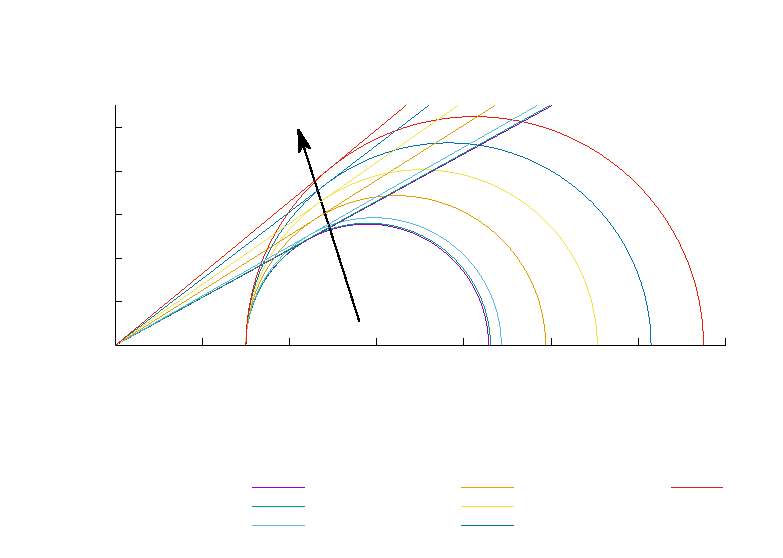
\includegraphics[width={360.00bp},height={252.00bp}]{Transitoire}}%
    \gplfronttext
  \end{picture}%
\endgroup

                                    \caption{Cercle transitore (pic)}
                                \end{figure}

                                    $\varphi = 28.77^\circ \div 39.53^\circ $


                                \begin{figure}
                                    \input{Résiduel.tex}
                                    \caption{Cercle résiduel ($\varepsilon_{yy} = 70\%$)}
                                \end{figure}
                                    $\varphi = 16.56^\circ \div 22.78^\circ $
                                    
\section{Comparaison des équations utilisées}

Expérimental : 
\[
I =  \frac{\dot{\varepsilon} \cdot \bar{a}}{\sqrt{\sigma_{33}/\rho_s}}; \quad \mu = \sin(\varphi)
\]

Simulation : 
\[
I = \dot{\varepsilon} \times \sqrt {\frac{m}{\sigma_{33}\times \bar{a}}}  
= \dot{\varepsilon} \times \sqrt {\frac{\frac{4}{3} \pi \frac{\bar{a}^3}{8} \times \rho_s}{\sigma_{33}\times \bar{a}}} 
= \dot{\varepsilon} \times \sqrt{\frac{\pi}{6}} \sqrt {\frac{\bar{a}^2 \rho_s}{\sigma_{33}}} 
= \boxed{\sqrt{\frac{\pi}{6}}} \times \frac{\dot{\varepsilon} \cdot \bar{a}}{\sqrt{\sigma_{33}/\rho_s}}
\]
\[
\mu = \tan(\varphi)
\]

\section{Rhéologie $\mu(I)$ résiduel}

\subsection{Première méthode}

La première méthode utilise les équations suivantes :
\[
\mu(I) = \mu_s + \frac{\mu_2 - \mu_s}{1 + \frac{I_0}{I}}
\]
\[
\Phi(I) = \Phi^{\max} - bI
\]

Les coefficients $\mu_s,\ \mu_2,\ I_0,\ \Phi_{\max},\ b$ sont déterminés empiriquement.

\begin{figure}
    \centering
    {\small
        % GNUPLOT: LaTeX picture with Postscript
\begingroup
  \makeatletter
  \providecommand\color[2][]{%
    \GenericError{(gnuplot) \space\space\space\@spaces}{%
      Package color not loaded in conjunction with
      terminal option `colourtext'%
    }{See the gnuplot documentation for explanation.%
    }{Either use 'blacktext' in gnuplot or load the package
      color.sty in LaTeX.}%
    \renewcommand\color[2][]{}%
  }%
  \providecommand\includegraphics[2][]{%
    \GenericError{(gnuplot) \space\space\space\@spaces}{%
      Package graphicx or graphics not loaded%
    }{See the gnuplot documentation for explanation.%
    }{The gnuplot epslatex terminal needs graphicx.sty or graphics.sty.}%
    \renewcommand\includegraphics[2][]{}%
  }%
  \providecommand\rotatebox[2]{#2}%
  \@ifundefined{ifGPcolor}{%
    \newif\ifGPcolor
    \GPcolortrue
  }{}%
  \@ifundefined{ifGPblacktext}{%
    \newif\ifGPblacktext
    \GPblacktextfalse
  }{}%
  % define a \g@addto@macro without @ in the name:
  \let\gplgaddtomacro\g@addto@macro
  % define empty templates for all commands taking text:
  \gdef\gplbacktext{}%
  \gdef\gplfronttext{}%
  \makeatother
  \ifGPblacktext
    % no textcolor at all
    \def\colorrgb#1{}%
    \def\colorgray#1{}%
  \else
    % gray or color?
    \ifGPcolor
      \def\colorrgb#1{\color[rgb]{#1}}%
      \def\colorgray#1{\color[gray]{#1}}%
      \expandafter\def\csname LTw\endcsname{\color{white}}%
      \expandafter\def\csname LTb\endcsname{\color{black}}%
      \expandafter\def\csname LTa\endcsname{\color{black}}%
      \expandafter\def\csname LT0\endcsname{\color[rgb]{1,0,0}}%
      \expandafter\def\csname LT1\endcsname{\color[rgb]{0,1,0}}%
      \expandafter\def\csname LT2\endcsname{\color[rgb]{0,0,1}}%
      \expandafter\def\csname LT3\endcsname{\color[rgb]{1,0,1}}%
      \expandafter\def\csname LT4\endcsname{\color[rgb]{0,1,1}}%
      \expandafter\def\csname LT5\endcsname{\color[rgb]{1,1,0}}%
      \expandafter\def\csname LT6\endcsname{\color[rgb]{0,0,0}}%
      \expandafter\def\csname LT7\endcsname{\color[rgb]{1,0.3,0}}%
      \expandafter\def\csname LT8\endcsname{\color[rgb]{0.5,0.5,0.5}}%
    \else
      % gray
      \def\colorrgb#1{\color{black}}%
      \def\colorgray#1{\color[gray]{#1}}%
      \expandafter\def\csname LTw\endcsname{\color{white}}%
      \expandafter\def\csname LTb\endcsname{\color{black}}%
      \expandafter\def\csname LTa\endcsname{\color{black}}%
      \expandafter\def\csname LT0\endcsname{\color{black}}%
      \expandafter\def\csname LT1\endcsname{\color{black}}%
      \expandafter\def\csname LT2\endcsname{\color{black}}%
      \expandafter\def\csname LT3\endcsname{\color{black}}%
      \expandafter\def\csname LT4\endcsname{\color{black}}%
      \expandafter\def\csname LT5\endcsname{\color{black}}%
      \expandafter\def\csname LT6\endcsname{\color{black}}%
      \expandafter\def\csname LT7\endcsname{\color{black}}%
      \expandafter\def\csname LT8\endcsname{\color{black}}%
    \fi
  \fi
    \setlength{\unitlength}{0.0500bp}%
    \ifx\gptboxheight\undefined%
      \newlength{\gptboxheight}%
      \newlength{\gptboxwidth}%
      \newsavebox{\gptboxtext}%
    \fi%
    \setlength{\fboxrule}{0.5pt}%
    \setlength{\fboxsep}{1pt}%
    \definecolor{tbcol}{rgb}{1,1,1}%
\begin{picture}(7200.00,5040.00)%
    \gplgaddtomacro\gplbacktext{%
      \csname LTb\endcsname%%
      \put(946,704){\makebox(0,0)[r]{\strut{}$0.28$}}%
      \csname LTb\endcsname%%
      \put(946,1161){\makebox(0,0)[r]{\strut{}$0.3$}}%
      \csname LTb\endcsname%%
      \put(946,1618){\makebox(0,0)[r]{\strut{}$0.32$}}%
      \csname LTb\endcsname%%
      \put(946,2076){\makebox(0,0)[r]{\strut{}$0.34$}}%
      \csname LTb\endcsname%%
      \put(946,2533){\makebox(0,0)[r]{\strut{}$0.36$}}%
      \csname LTb\endcsname%%
      \put(946,2990){\makebox(0,0)[r]{\strut{}$0.38$}}%
      \csname LTb\endcsname%%
      \put(946,3447){\makebox(0,0)[r]{\strut{}$0.4$}}%
      \csname LTb\endcsname%%
      \put(946,3905){\makebox(0,0)[r]{\strut{}$0.42$}}%
      \csname LTb\endcsname%%
      \put(946,4362){\makebox(0,0)[r]{\strut{}$0.44$}}%
      \csname LTb\endcsname%%
      \put(946,4819){\makebox(0,0)[r]{\strut{}$0.46$}}%
      \csname LTb\endcsname%%
      \put(1078,484){\makebox(0,0){\strut{}$10^{-4}$}}%
      \csname LTb\endcsname%%
      \put(2986,484){\makebox(0,0){\strut{}$10^{-3}$}}%
      \csname LTb\endcsname%%
      \put(4895,484){\makebox(0,0){\strut{}$10^{-2}$}}%
      \csname LTb\endcsname%%
      \put(6803,484){\makebox(0,0){\strut{}$10^{-1}$}}%
      \put(1651,3996){\makebox(0,0)[l]{\strut{}$\mu_s = 0.2953$}}%
      \put(1651,3585){\makebox(0,0)[l]{\strut{}$\mu_2 = 0.5329$}}%
      \put(1651,3173){\makebox(0,0)[l]{\strut{}$I_0 = 0.0483$}}%
    }%
    \gplgaddtomacro\gplfronttext{%
      \csname LTb\endcsname%%
      \put(209,2761){\rotatebox{-270}{\makebox(0,0){\strut{}$\mu$}}}%
      \put(3940,154){\makebox(0,0){\strut{}$I$}}%
      \csname LTb\endcsname%%
      \put(3322,4646){\makebox(0,0)[r]{\strut{}Données}}%
      \csname LTb\endcsname%%
      \put(3322,4426){\makebox(0,0)[r]{\strut{}$\mu(I)$ régression}}%
    }%
    \gplbacktext
    \put(0,0){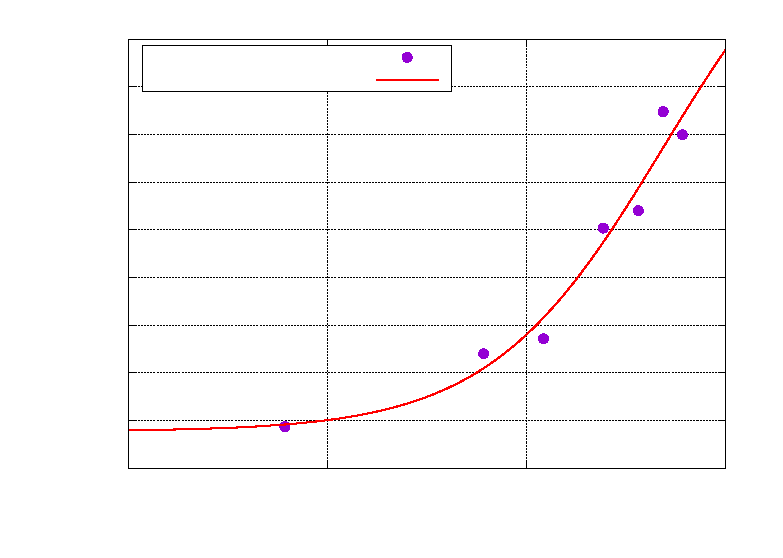
\includegraphics[width={360.00bp},height={252.00bp}]{./mu_I_fit}}%
    \gplfronttext
  \end{picture}%
\endgroup

    }
    \caption{$\mu(I)$ ($\varepsilon_{yy} = 70\%$)}
\end{figure}

\begin{figure}
    \centering
    {\small
        % GNUPLOT: LaTeX picture with Postscript
\begingroup
  \makeatletter
  \providecommand\color[2][]{%
    \GenericError{(gnuplot) \space\space\space\@spaces}{%
      Package color not loaded in conjunction with
      terminal option `colourtext'%
    }{See the gnuplot documentation for explanation.%
    }{Either use 'blacktext' in gnuplot or load the package
      color.sty in LaTeX.}%
    \renewcommand\color[2][]{}%
  }%
  \providecommand\includegraphics[2][]{%
    \GenericError{(gnuplot) \space\space\space\@spaces}{%
      Package graphicx or graphics not loaded%
    }{See the gnuplot documentation for explanation.%
    }{The gnuplot epslatex terminal needs graphicx.sty or graphics.sty.}%
    \renewcommand\includegraphics[2][]{}%
  }%
  \providecommand\rotatebox[2]{#2}%
  \@ifundefined{ifGPcolor}{%
    \newif\ifGPcolor
    \GPcolortrue
  }{}%
  \@ifundefined{ifGPblacktext}{%
    \newif\ifGPblacktext
    \GPblacktextfalse
  }{}%
  % define a \g@addto@macro without @ in the name:
  \let\gplgaddtomacro\g@addto@macro
  % define empty templates for all commands taking text:
  \gdef\gplbacktext{}%
  \gdef\gplfronttext{}%
  \makeatother
  \ifGPblacktext
    % no textcolor at all
    \def\colorrgb#1{}%
    \def\colorgray#1{}%
  \else
    % gray or color?
    \ifGPcolor
      \def\colorrgb#1{\color[rgb]{#1}}%
      \def\colorgray#1{\color[gray]{#1}}%
      \expandafter\def\csname LTw\endcsname{\color{white}}%
      \expandafter\def\csname LTb\endcsname{\color{black}}%
      \expandafter\def\csname LTa\endcsname{\color{black}}%
      \expandafter\def\csname LT0\endcsname{\color[rgb]{1,0,0}}%
      \expandafter\def\csname LT1\endcsname{\color[rgb]{0,1,0}}%
      \expandafter\def\csname LT2\endcsname{\color[rgb]{0,0,1}}%
      \expandafter\def\csname LT3\endcsname{\color[rgb]{1,0,1}}%
      \expandafter\def\csname LT4\endcsname{\color[rgb]{0,1,1}}%
      \expandafter\def\csname LT5\endcsname{\color[rgb]{1,1,0}}%
      \expandafter\def\csname LT6\endcsname{\color[rgb]{0,0,0}}%
      \expandafter\def\csname LT7\endcsname{\color[rgb]{1,0.3,0}}%
      \expandafter\def\csname LT8\endcsname{\color[rgb]{0.5,0.5,0.5}}%
    \else
      % gray
      \def\colorrgb#1{\color{black}}%
      \def\colorgray#1{\color[gray]{#1}}%
      \expandafter\def\csname LTw\endcsname{\color{white}}%
      \expandafter\def\csname LTb\endcsname{\color{black}}%
      \expandafter\def\csname LTa\endcsname{\color{black}}%
      \expandafter\def\csname LT0\endcsname{\color{black}}%
      \expandafter\def\csname LT1\endcsname{\color{black}}%
      \expandafter\def\csname LT2\endcsname{\color{black}}%
      \expandafter\def\csname LT3\endcsname{\color{black}}%
      \expandafter\def\csname LT4\endcsname{\color{black}}%
      \expandafter\def\csname LT5\endcsname{\color{black}}%
      \expandafter\def\csname LT6\endcsname{\color{black}}%
      \expandafter\def\csname LT7\endcsname{\color{black}}%
      \expandafter\def\csname LT8\endcsname{\color{black}}%
    \fi
  \fi
    \setlength{\unitlength}{0.0500bp}%
    \ifx\gptboxheight\undefined%
      \newlength{\gptboxheight}%
      \newlength{\gptboxwidth}%
      \newsavebox{\gptboxtext}%
    \fi%
    \setlength{\fboxrule}{0.5pt}%
    \setlength{\fboxsep}{1pt}%
    \definecolor{tbcol}{rgb}{1,1,1}%
\begin{picture}(7200.00,5040.00)%
    \gplgaddtomacro\gplbacktext{%
      \csname LTb\endcsname%%
      \put(1078,704){\makebox(0,0)[r]{\strut{}$0.555$}}%
      \csname LTb\endcsname%%
      \put(1078,1116){\makebox(0,0)[r]{\strut{}$0.56$}}%
      \csname LTb\endcsname%%
      \put(1078,1527){\makebox(0,0)[r]{\strut{}$0.565$}}%
      \csname LTb\endcsname%%
      \put(1078,1939){\makebox(0,0)[r]{\strut{}$0.57$}}%
      \csname LTb\endcsname%%
      \put(1078,2350){\makebox(0,0)[r]{\strut{}$0.575$}}%
      \csname LTb\endcsname%%
      \put(1078,2762){\makebox(0,0)[r]{\strut{}$0.58$}}%
      \csname LTb\endcsname%%
      \put(1078,3173){\makebox(0,0)[r]{\strut{}$0.585$}}%
      \csname LTb\endcsname%%
      \put(1078,3585){\makebox(0,0)[r]{\strut{}$0.59$}}%
      \csname LTb\endcsname%%
      \put(1078,3996){\makebox(0,0)[r]{\strut{}$0.595$}}%
      \csname LTb\endcsname%%
      \put(1078,4408){\makebox(0,0)[r]{\strut{}$0.6$}}%
      \csname LTb\endcsname%%
      \put(1078,4819){\makebox(0,0)[r]{\strut{}$0.605$}}%
      \csname LTb\endcsname%%
      \put(1210,484){\makebox(0,0){\strut{}$10^{-4}$}}%
      \csname LTb\endcsname%%
      \put(3074,484){\makebox(0,0){\strut{}$10^{-3}$}}%
      \csname LTb\endcsname%%
      \put(4939,484){\makebox(0,0){\strut{}$10^{-2}$}}%
      \csname LTb\endcsname%%
      \put(6803,484){\makebox(0,0){\strut{}$10^{-1}$}}%
      \put(1769,1733){\makebox(0,0)[l]{\strut{}$\Phi_{max} = 0.6019$}}%
      \put(1769,1321){\makebox(0,0)[l]{\strut{}$b = 0.4641$}}%
    }%
    \gplgaddtomacro\gplfronttext{%
      \csname LTb\endcsname%%
      \put(209,2761){\rotatebox{-270}{\makebox(0,0){\strut{}$\Phi$}}}%
      \put(4006,154){\makebox(0,0){\strut{}$I$}}%
      \csname LTb\endcsname%%
      \put(3454,1097){\makebox(0,0)[r]{\strut{}Données}}%
      \csname LTb\endcsname%%
      \put(3454,877){\makebox(0,0)[r]{\strut{}$\Phi(I)$ régression}}%
    }%
    \gplbacktext
    \put(0,0){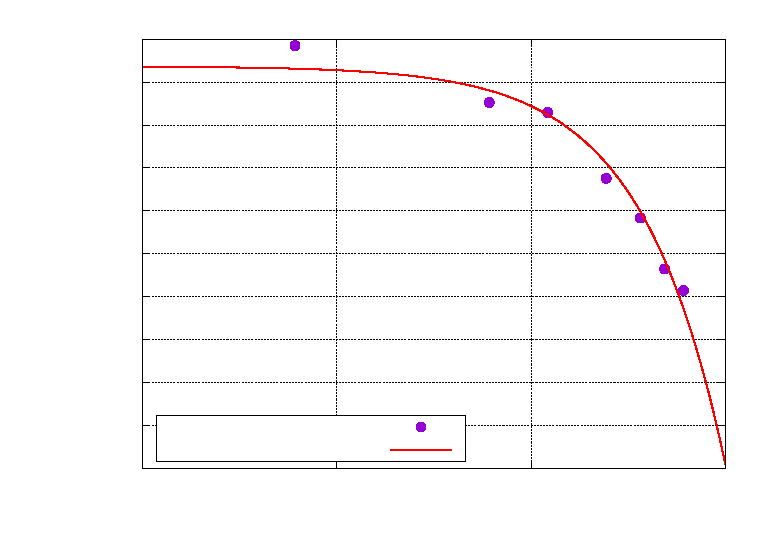
\includegraphics[width={360.00bp},height={252.00bp}]{./Pack_I_fit}}%
    \gplfronttext
  \end{picture}%
\endgroup

    }
    \caption{$\Phi(I)$ ($\varepsilon_{yy} = 70\%$)}
\end{figure}

\subsection{Deuxième méthode}

La deuxième méthode, proposée dans l'article 
\href{https://link-springer-com.sid2nomade-1.grenet.fr/article/10.1007/s10035-024-01459-7}{Scaling laws for quasi-statically deforming granular soil at critical state [2024] (Fei, Jianbo et al.)}, 
introduit un nombre d'inertie quasi-statique $Q$ qui tient compte du degré de compaction $\Phi_0$ :

\[
Q = \left[ \Phi_0  \ln \left( I \right) + \alpha \right]
\]
où $\alpha = 30$.

\[
\mu = \xi Q + C
\]

Les coefficients $\xi,\ C,\ \Phi_0$ sont déterminés empiriquement ($\xi \approx 0.06$ et $C \approx 0.2$).

\begin{figure}
    \centering
    {\small
        % GNUPLOT: LaTeX picture with Postscript
\begingroup
  \makeatletter
  \providecommand\color[2][]{%
    \GenericError{(gnuplot) \space\space\space\@spaces}{%
      Package color not loaded in conjunction with
      terminal option `colourtext'%
    }{See the gnuplot documentation for explanation.%
    }{Either use 'blacktext' in gnuplot or load the package
      color.sty in LaTeX.}%
    \renewcommand\color[2][]{}%
  }%
  \providecommand\includegraphics[2][]{%
    \GenericError{(gnuplot) \space\space\space\@spaces}{%
      Package graphicx or graphics not loaded%
    }{See the gnuplot documentation for explanation.%
    }{The gnuplot epslatex terminal needs graphicx.sty or graphics.sty.}%
    \renewcommand\includegraphics[2][]{}%
  }%
  \providecommand\rotatebox[2]{#2}%
  \@ifundefined{ifGPcolor}{%
    \newif\ifGPcolor
    \GPcolortrue
  }{}%
  \@ifundefined{ifGPblacktext}{%
    \newif\ifGPblacktext
    \GPblacktextfalse
  }{}%
  % define a \g@addto@macro without @ in the name:
  \let\gplgaddtomacro\g@addto@macro
  % define empty templates for all commands taking text:
  \gdef\gplbacktext{}%
  \gdef\gplfronttext{}%
  \makeatother
  \ifGPblacktext
    % no textcolor at all
    \def\colorrgb#1{}%
    \def\colorgray#1{}%
  \else
    % gray or color?
    \ifGPcolor
      \def\colorrgb#1{\color[rgb]{#1}}%
      \def\colorgray#1{\color[gray]{#1}}%
      \expandafter\def\csname LTw\endcsname{\color{white}}%
      \expandafter\def\csname LTb\endcsname{\color{black}}%
      \expandafter\def\csname LTa\endcsname{\color{black}}%
      \expandafter\def\csname LT0\endcsname{\color[rgb]{1,0,0}}%
      \expandafter\def\csname LT1\endcsname{\color[rgb]{0,1,0}}%
      \expandafter\def\csname LT2\endcsname{\color[rgb]{0,0,1}}%
      \expandafter\def\csname LT3\endcsname{\color[rgb]{1,0,1}}%
      \expandafter\def\csname LT4\endcsname{\color[rgb]{0,1,1}}%
      \expandafter\def\csname LT5\endcsname{\color[rgb]{1,1,0}}%
      \expandafter\def\csname LT6\endcsname{\color[rgb]{0,0,0}}%
      \expandafter\def\csname LT7\endcsname{\color[rgb]{1,0.3,0}}%
      \expandafter\def\csname LT8\endcsname{\color[rgb]{0.5,0.5,0.5}}%
    \else
      % gray
      \def\colorrgb#1{\color{black}}%
      \def\colorgray#1{\color[gray]{#1}}%
      \expandafter\def\csname LTw\endcsname{\color{white}}%
      \expandafter\def\csname LTb\endcsname{\color{black}}%
      \expandafter\def\csname LTa\endcsname{\color{black}}%
      \expandafter\def\csname LT0\endcsname{\color{black}}%
      \expandafter\def\csname LT1\endcsname{\color{black}}%
      \expandafter\def\csname LT2\endcsname{\color{black}}%
      \expandafter\def\csname LT3\endcsname{\color{black}}%
      \expandafter\def\csname LT4\endcsname{\color{black}}%
      \expandafter\def\csname LT5\endcsname{\color{black}}%
      \expandafter\def\csname LT6\endcsname{\color{black}}%
      \expandafter\def\csname LT7\endcsname{\color{black}}%
      \expandafter\def\csname LT8\endcsname{\color{black}}%
    \fi
  \fi
    \setlength{\unitlength}{0.0500bp}%
    \ifx\gptboxheight\undefined%
      \newlength{\gptboxheight}%
      \newlength{\gptboxwidth}%
      \newsavebox{\gptboxtext}%
    \fi%
    \setlength{\fboxrule}{0.5pt}%
    \setlength{\fboxsep}{1pt}%
    \definecolor{tbcol}{rgb}{1,1,1}%
\begin{picture}(7200.00,5040.00)%
    \gplgaddtomacro\gplbacktext{%
      \csname LTb\endcsname%%
      \put(946,704){\makebox(0,0)[r]{\strut{}$0.24$}}%
      \csname LTb\endcsname%%
      \put(946,1218){\makebox(0,0)[r]{\strut{}$0.26$}}%
      \csname LTb\endcsname%%
      \put(946,1733){\makebox(0,0)[r]{\strut{}$0.28$}}%
      \csname LTb\endcsname%%
      \put(946,2247){\makebox(0,0)[r]{\strut{}$0.3$}}%
      \csname LTb\endcsname%%
      \put(946,2762){\makebox(0,0)[r]{\strut{}$0.32$}}%
      \csname LTb\endcsname%%
      \put(946,3276){\makebox(0,0)[r]{\strut{}$0.34$}}%
      \csname LTb\endcsname%%
      \put(946,3790){\makebox(0,0)[r]{\strut{}$0.36$}}%
      \csname LTb\endcsname%%
      \put(946,4305){\makebox(0,0)[r]{\strut{}$0.38$}}%
      \csname LTb\endcsname%%
      \put(946,4819){\makebox(0,0)[r]{\strut{}$0.4$}}%
      \csname LTb\endcsname%%
      \put(1078,484){\makebox(0,0){\strut{}$10.5$}}%
      \csname LTb\endcsname%%
      \put(2032,484){\makebox(0,0){\strut{}$11$}}%
      \csname LTb\endcsname%%
      \put(2986,484){\makebox(0,0){\strut{}$11.5$}}%
      \csname LTb\endcsname%%
      \put(3941,484){\makebox(0,0){\strut{}$12$}}%
      \csname LTb\endcsname%%
      \put(4895,484){\makebox(0,0){\strut{}$12.5$}}%
      \csname LTb\endcsname%%
      \put(5849,484){\makebox(0,0){\strut{}$13$}}%
      \csname LTb\endcsname%%
      \put(6803,484){\makebox(0,0){\strut{}$13.5$}}%
      \put(1651,3996){\makebox(0,0)[l]{\strut{}$\xi = 0.0485$}}%
      \put(1651,3585){\makebox(0,0)[l]{\strut{}$c = -0.2636$}}%
      \put(1651,3173){\makebox(0,0)[l]{\strut{}$\Phi_0 = 0.4868$}}%
    }%
    \gplgaddtomacro\gplfronttext{%
      \csname LTb\endcsname%%
      \put(209,2761){\rotatebox{-270}{\makebox(0,0){\strut{}$\mu$}}}%
      \put(3940,154){\makebox(0,0){\strut{}$Q$}}%
      \csname LTb\endcsname%%
      \put(3322,4646){\makebox(0,0)[r]{\strut{}Données}}%
      \csname LTb\endcsname%%
      \put(3322,4426){\makebox(0,0)[r]{\strut{}$\mu(Q)$ régression}}%
    }%
    \gplbacktext
    \put(0,0){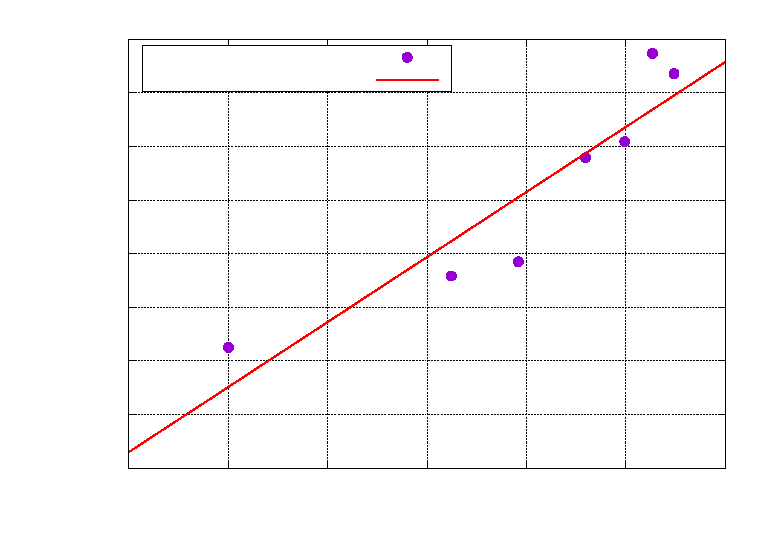
\includegraphics[width={360.00bp},height={252.00bp}]{./Q_mu}}%
    \gplfronttext
  \end{picture}%
\endgroup

    }
    \caption{$\mu(Q)$ avec $Q = f(\Phi_0, I)$}
\end{figure}

\bibliographystyle{plain}
\bibliography{Bibliographie}


\end{document}


